%# -*- coding: utf-8-unix -*-
%%==================================================
%% thesis.tex
%%==================================================

% 双面打印
% \documentclass[doctor, fontset=adobe, openright, twoside]{sjtuthesis}
% \documentclass[bachelor, fontset=adobe, openany, oneside, submit]{sjtuthesis}
\documentclass[master, fontset=adobe, twoside, review]{sjtuthesis}
% \documentclass[%
%   bachelor|master|doctor,	% 必选项
%   fontset=adobe|windows,  	% 只测试了adobe
%   oneside|twoside,		% 单面打印,双面打印(奇偶页交换页边距,默认)
%   openany|openright, 		% 可以在奇数或者偶数页开新章|只在奇数页开新章(默认)
%   zihao=-4|5,, 		% 正文字号:小四、五号(默认)
%   review,	 		% 盲审论文,隐去作者姓名、学号、导师姓名、致谢、发表论文和参与的项目
%   submit			% 定稿提交的论文,插入签名扫描版的原创性声明、授权声明
% ]

% 逐个导入参考文献数据库
\addbibresource{bib/thesis.bib}
% \addbibresource{bib/chap2.bib}

\begin{document}

%% 无编号内容:中英文论文封面、授权页
%# -*- coding: utf-8-unix -*-
\title{分布式并行计算框架的shuffle优化}
\author{付周望}
\advisor{戚正伟教授}
% \coadvisor{某某教授}
\defenddate{2018年1月15日}
\school{上海交通大学}
\institute{软件学院}
\studentnumber{115037910032}
\major{软件工程}

\englishtitle{Efficient Shuffle Management with SCache for DAG
Computing Frameworks}
\englishauthor{\textsc{Zhouwang Fu}}
\englishadvisor{Prof. \textsc{Zhengwei Qi}}
% \englishcoadvisor{Prof. \textsc{Uom Uom}}
\englishschool{Shanghai Jiao Tong University}
\englishinstitute{\textsc{School of Software} \\
  \textsc{Shanghai Jiao Tong University} \\
  \textsc{Shanghai, P.R.China}}
\englishmajor{Software Engineering}
\englishdate{Jan, 2018}


\maketitle

\makeenglishtitle

\makeatletter
\ifsjtu@submit\relax
	
\includepdf{pdf/original.pdf}
	\cleardoublepage
	
\includepdf{pdf/authorization.pdf}
	\cleardoublepage
\else
\ifsjtu@review\relax
% exclude the original claim and authorization
\else
	\makeDeclareOriginal
	\makeDeclareAuthorization
\fi
\fi
\makeatother


\frontmatter 	% 使用罗马数字对前言编号

%% 摘要
\pagestyle{main}
%# -*- coding: utf-8-unix -*-
%%==================================================
%% abstract.tex for SJTU Master Thesis
%%==================================================

\begin{abstract}

大数据时代的到来使得分布式计算变得越来越普及。
为了快速地处理大规模的数据,有大量复杂的分布式并行计算框架被设计并使用,比如Hadoop MapReduce\cite{hadoop},Spark\cite{apachespark},Dryad\cite{dryad}, Tez\cite{tez}等。
这些分布式计算框架大多采用将用户计算逻辑用有向无环图(Directed Acyclic Graph, DAG)的方式呈现出来。
在执行DAG的每一个计算阶段时,这些计算框架大多采用了整体同步并行计算模型(Bulk-Synchronous Parallel, BSP)来对大数据进行分布式的并行批处理。

在这些相邻的计算阶段之间,shuffle,或者说跨网络的多对多分块数据的读写满足了计算逻辑对于不同数据的依赖。与此同时,shuffle的过程也带来了大量的网络数据传输。
受限于计算对于数据的依赖以及网络,磁盘等硬件性能,使得依赖于shuffle的这些任务的性能会因为shuffle的开销而受到巨大损失。
尤其是在一些需要大量shuffle数据的情境中,比如两张数据库大表的交集,shuffle的开销甚至会成为整个应用的性能瓶颈。
更重要的是,这个问题在大多数分布式并行计算框架中都普遍存在。

为了提供一种具有普遍意义的shuffle优化方案,本研究抽取了这些系统在shuffle设计中存在的一些共性问题:1)粗粒度的硬件资源管理降低了资源的可复用性, 比如使得计算资源在进行I/O操作时长时间闲置。
2)同步滞后的shuffle读取不仅增加了计算任务执行过程中对shuffle网络传输的显式等待时间,也给网络带来一个瞬时的流量高峰,进一步减慢了网络传输过程。

针对以上问题,本文提出了S(huffle)Cache --- 一个开源的即用型系统来优化DAG计算过程中的shuffle阶段。
通过在计算阶段真正执行前提取表达计算逻辑的DAG以及其中的shuffle依赖关系,SCache可以将shuffle过程从DAG计算过程中解耦合,从而提供更细粒度的硬件资源管理,提高资源利用率和复用率。
与此同时,SCache通过提前异步的shuffle传输来隐藏任务计算过程中显式的网络等待时间,同时也减缓了shuffle给网络带来的压力。
此外,SCache还利用结合应用上下文的内存管理,来实现对shuffle数据的内存缓存,进一步提升shuffle过程的效率。
为了实现以上的优化目标,本研究做出了以下主要贡献:

\begin{enumerate}
    \item 将shuffle过程从计算过程中解耦,使得shuffle过程独立到外部进行管理,从而实现了更细粒度的硬件资源管理。
    \item 结合应用的上下文对shuffle数据进行预取,既避免了同步数据读取给网络带来的压力,又能将大部分网络传输时间隐藏到计算阶段。
    \item 结合应用的上下文对shuffle数据内存管理和内存缓存,进一步提升shuffle过程的效率。
    \item 根据现有的分布式计算框架shuffle的特点设计了相应的接口(API)。通用的接口设计使得优化能被应用到不同的分布式并行计算框架当中。
\end{enumerate}

基于以上阐述,本研究课题实现了SCache,同时修改了Apache Spark对SCache进行适配。
并且通过仿真实验和Amazon AWS EC2集群上大规模数据测试来验证其优化效果。
在不同的数据集和测试程序的测试中,SCache能减少将近89\%的shuffle开销。
在TPC-DS的测试中,SCache的优化能给分布式SQL查询带来平均大约40\%的性能提升。

\keywords{\large 分布式DAG计算框架, Shuffle, 优化}
\end{abstract}

\begin{englishabstract}

Recent years have witnessed the widespread use of distributed computing in the big data area.
Numbers of sophisticated distributed data parallel computing frameworks, such as Hadoop MapReduce\cite{hadoop}, Spark\cite{apachespark}, Dryad\cite{dryad}, and Tez\cite{tez},
have been developed and deployed to accelerate the big data processing.
Most of these frameworks do the computing by transforming the application logic into Directed Acyclic Graph (DAG).
In order to increase the parallelism, each computing stage is usually managed according to the Bulk-Synchronous Parallel (BSP) model during the execution of DAG.

Shuffle, or the cross-network read and aggregation of partitioned data among tasks with data dependencies in the consecutive execution stages, 
usually brings in large network transfer. 
Due to the dependency constrains and the limited performance of disks and networks, execution of those descendant tasks could be delayed by inefficient shuffles. 
This delay can further slow down the whole application process. 
The performance degradation introduced by shuffle can become overwhelming in the shuffle intensive applications such as a join of two big tables.
Moreover, the above deficiencies of shuffle generally exist in most of the DAG data parallel computing frameworks. 
In this paper, we extract the common issues in current shuffle mechanism: 
1) The coarse granularity resource management decreases the utilization and multiplexing of hardware resources. For example, the inefficient management can keep CPU idle while tasks doing I/O operations.
2)The synchronized shuffle read increases the explicit network waiting time during task execution and brings a network burst which further slows down the shuffle read itself.

Based on the above observations, we present S(huffle)Cache --- an open source plug-in system that particularly focuses on shuffle optimization in frameworks defining jobs as DAGs. 
By extracting and analyzing the DAGs and shuffle dependencies prior to the actual task execution, 
SCache can take full advantage of the fine granularity resource management and system memory to accelerate the shuffle process. 
Meanwhile, SCache manages the shuffle data out of the frameworks and transfers data asynchronously, which helps overlap the network transfer time and avoid network burst.
In addition, SCache provides an application-context-aware in-memory shuffle data management scheme to further accelerate the shuffle process.  
In order to achieve the optimizations, we make following contributions:

\begin{enumerate}
    \item Decouple the shuffles and manage them out of the DAG data parallel computing frameworks so that the shuffle data management can become more efficient.
    \item Implement the shuffle data pre-fetch with application context so that the network burst can be avoided and the network transfer time can be overlapped in execution phases.
    \item Implement the application-context-aware in-memory shuffle data management to accelerate the shuffle process.
    \item Design and implement the general APIs for the DAG data parallel computing frameworks so that the optimizations can be applied easily.
\end{enumerate}

We have implemented SCache and customized Spark to use it as the external shuffle service and co-scheduler. 
The performance of SCache is evaluated with both simulations and testbed experiments on a 50-node Amazon EC2 cluster.
Those evaluations have demonstrated that, by incorporating SCache, the shuffle overhead of Spark can be reduced by nearly 89\%, 
and the overall completion time of TPC-DS queries improves 40\% on average.


\englishkeywords{\large Distributed DAG frameworks, Shuffle, Optimization}
\end{englishabstract}



%% 目录、插图目录、表格目录
\tableofcontents
\listoffigures
\addcontentsline{toc}{chapter}{\listfigurename} %将插图目录加入全文目录
\listoftables
\addcontentsline{toc}{chapter}{\listtablename}  %将表格目录加入全文目录
\listofalgorithms
\addcontentsline{toc}{chapter}{算法索引}        %将算法目录加入全文目录

%# -*- coding: utf-8-unix -*-
\chapter{主要符号对照表}
\label{chap:symb}

\begin{longtable}{rl}
$\epsilon$     & 介电常数 \\
 $\mu$ 		& 磁导率 \\
 $\epsilon$     & 介电常数 \\
 $\mu$ 		& 磁导率 \\
 $\epsilon$     & 介电常数 \\
 $\mu$ 		& 磁导率 \\
 $\epsilon$ 	& 介电常数 \\
 $\mu$ 		& 磁导率 \\
 $\epsilon$     & 介电常数 \\
 $\mu$ 		& 磁导率 \\
 $\epsilon$     & 介电常数 \\
 $\mu$ 		& 磁导率 \\
 $\epsilon$     & 介电常数 \\
 $\mu$ 		& 磁导率 \\
 $\epsilon$ 	& 介电常数 \\
 $\mu$ 		& 磁导率 \\
 $\epsilon$     & 介电常数 \\
 $\mu$ 		& 磁导率 \\
 $\epsilon$     & 介电常数 \\
 $\mu$ 		& 磁导率 \\
 $\epsilon$     & 介电常数 \\
 $\mu$ 		& 磁导率 \\
 $\epsilon$ 	& 介电常数 \\
 $\mu$ 		& 磁导率 \\
 $\epsilon$     & 介电常数 \\
 $\mu$ 		& 磁导率 \\
 $\epsilon$     & 介电常数 \\
 $\mu$ 		& 磁导率 \\
 $\epsilon$     & 介电常数 \\
 $\mu$ 		& 磁导率 \\
 $\epsilon$ 	& 介电常数 \\
 $\mu$ 		& 磁导率 \\
 $\epsilon$     & 介电常数 \\
 $\mu$ 		& 磁导率 \\
 $\epsilon$     & 介电常数 \\
 $\mu$ 		& 磁导率 \\
 $\epsilon$     & 介电常数 \\
 $\mu$ 		& 磁导率 \\
 $\epsilon$ 	& 介电常数 \\
 $\mu$ 		& 磁导率 \\
 $\epsilon$     & 介电常数 \\
 $\mu$ 		& 磁导率 \\
 $\epsilon$     & 介电常数 \\
 $\mu$ 		& 磁导率 \\
 $\epsilon$     & 介电常数 \\
 $\mu$ 		& 磁导率 \\
 $\epsilon$ 	& 介电常数 \\
 $\mu$ 		& 磁导率 \\
 $\epsilon$     & 介电常数 \\
 $\mu$ 		& 磁导率 \\
 $\epsilon$     & 介电常数 \\
 $\mu$ 		& 磁导率 \\
 $\epsilon$     & 介电常数 \\
 $\mu$ 		& 磁导率 \\
\end{longtable}
 % 主要符号、缩略词对照表

\mainmatter	% 使用阿拉伯数字对正文编号

%% 正文内容
\pagestyle{main}
\section{Introduction}
\ifrevision
\reversemarginpar
\marginnote{60D}
\fi
Recent years have witnessed widespread use of sophisticated frameworks, such as Hadoop MapReduce \cite{hadoop}, Dryad \cite{dryad}, Spark \cite{spark}, and Apache Tez \cite{tez}.
\hlyellow{
Most of them define jobs as directed acyclic graphs (DAGs), such as map-reduce pipeline in Hadoop MapReduce, lineage of resilient distributed datasets (RDD) in Spark, vertices and edges in Dryad and Tez, etc.
}
Despite the differences among data-intensive frameworks, their communication is always structured as a shuffle phase,  which takes place between successive computation stages. 
Such shuffle phase places significant burden for both the disk and network I/O, thus heavily affecting the end-to-end application performance. 
For instance, a MapReduce trace analysis from Facebook shows that shuffle accounts for 33\% of the job completion time on average, and up to 70\% in shuffle-heavy jobs \cite{managing}.

Although continued efforts of performance optimization have been made among a variety of computing frameworks \cite{sync, babu, tachyon, pacman, quincy, delay}, 
the shuffle is often poorly optimized in practice.
% take over shuffle
%shuffle characteristic
In particular, we observe that one major deficiency lies in a lack of fine-grained, coordinated management among different system resources.
%In the current practice, the shuffle phase is often split into two parts --- \textit{shuffle read} and \textit{shuffle write}. 
As Figure \ref{fig:workflow} shows, the \textit{shuffle write} is responsible for writing intermediate results to disk, which is attached to the tasks in ancestor stage (i.e., map task).  
And the \textit{shuffle read} fetches intermediate results from remote disks through network, which is commonly integrated as part of the tasks in descendant stage (i.e., reduce task). 
Once scheduled, a fixed bundle of resources (i.e., CPU, memory, disk and network) named \textit{slot} is assigned to each of the computation task, and the resources are released only after the task finishes.
Such task aggregation together with the coarse-grained scheduling effectively simplifies task management.
\hlyellow{
However, since a cluster has a limited number of slots, attaching the I/O intensive shuffle phase to the CPU/memory intensive computation phase results in a poor multiplexing between computational and I/O resources.
}
%The map task in Figure \ref{fig:workflow} well explains such deficiency: the I/O resource allocated to the stage is always idle during the computation time, and the computation/memory resource is totally wasted during the shuffle write attached to it, and vice versa.
\begin{figure}
	\centering
	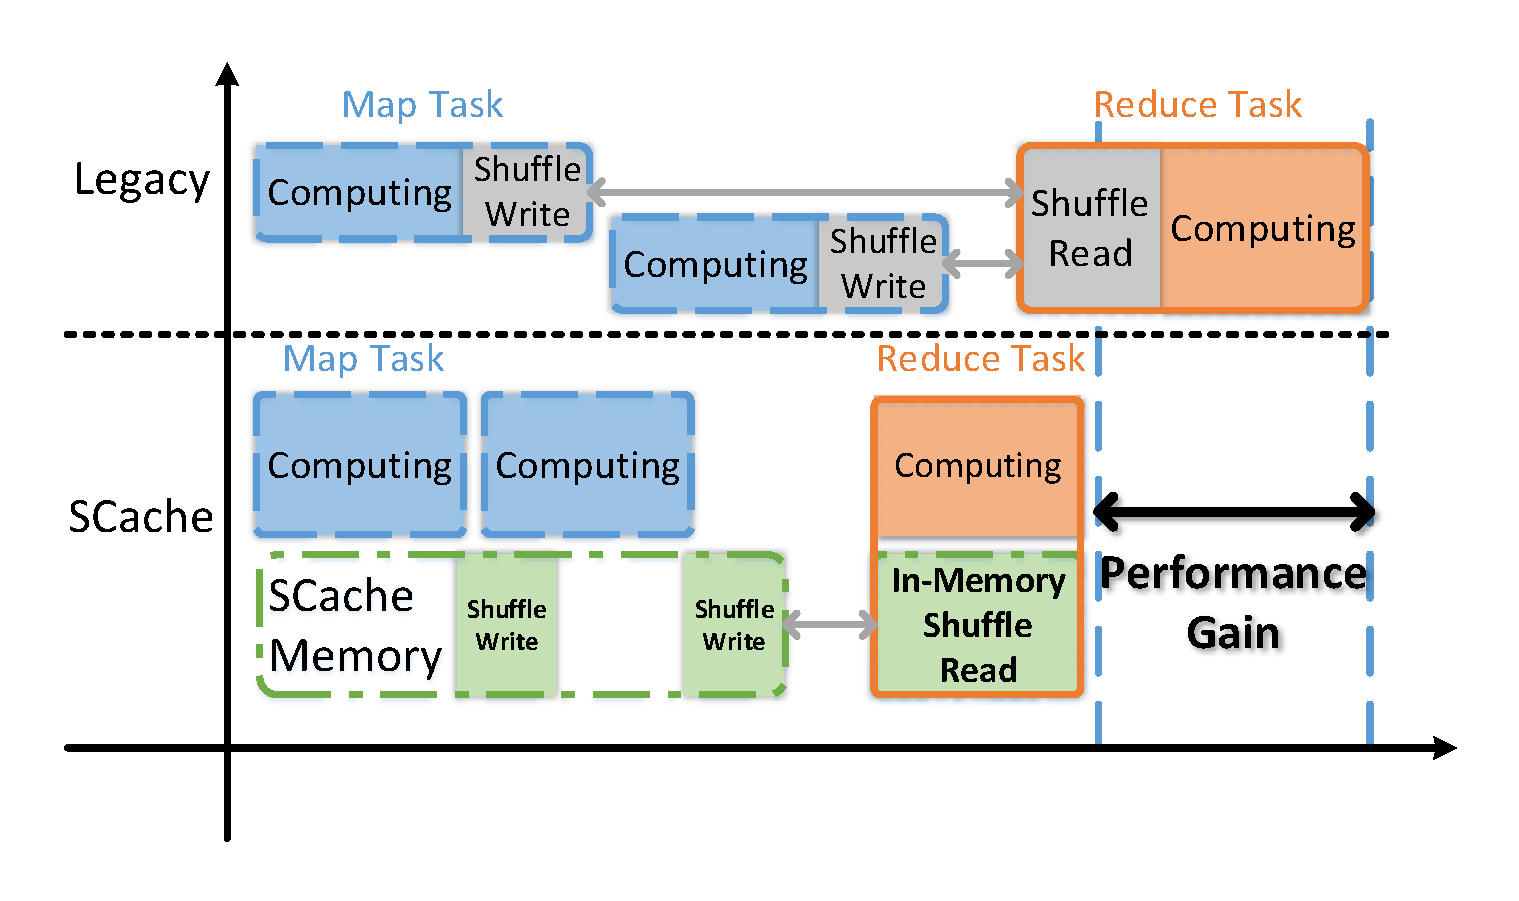
\includegraphics[width=\linewidth]{fig/workflow}
	\caption{Workflow Comparison between Legacy DAG Computing Frameworks and Frameworks with SCache}
	\label{fig:workflow}
	\vspace{-1em}
\end{figure}

Moreover, the shuffle read phase introduces all-to-all communication pattern across the network, and such network I/O procedure is also poorly coordinated.
Note that the shuffle read phase starts fetching data only after the corresponding reduce tasks start.
Meanwhile, the reduce tasks belonging to a same execution phase are scheduled at the same time by default. 
As a result, all the corresponding reduce tasks start fetching shuffle data almost simultaneously.
Such synchronized network communication causes a burst demand for network I/O, which in turn greatly enlarges the shuffle read completion time. 
To desynchronize the network communication, an intuitive way is to launch some tasks in the descendent stage earlier, such as "slow-start" from Hadoop MapReduce\cite{hadoop}. 
However, such early-start is by no means a panacea. 
\hlyellow{
This is because the early-start always introduces an extra early allocation of slot, which slows down the current stage execution.
}
% This is because although the reduce tasks can start fetching data earlier, the computation can only take place after all the data is ready. 

%In one word, existing solutions suffer from either inefficient use of network I/O, or a waste of computational resources (i.e., CPU and memory) caused by task pre-launching.

%For example, Apache Hadoop \cite{hadoop} provides an \emph{early start} mechanism that launches reduce tasks after a certain portion (5\% by default) of map tasks has completed, which is adopted in many of the recent works \cite{ihadoop, ishuffle, dynmr}.
% DAG computing framworks deriving from MapReduce \cite{mapreduce} contains a hard barrier between computing stages. The terminology of this barrier is \textit{shuffle}. Shuffle contains two parts on the connecting stages -- \textit{shuffle write} and \textit{shuffle read}. On the side of ancestor stages, \textit{shuffle write} is resoponsible for writing intermediate results to disk. On the side of descendant stage, \textit{shuffle read} fetches intermediate results from remote disks through network. Although highly optimized in other factors, the shuffle of framework is still primitive.  The coarse design of shuffle introduce a significiant performance overhead.
% % design inconsistent
% For instance, a MapReduce trace analysis from Facebook shows that shuffle accounts for 33\% JCT on average, up to 70\% in shuffle-heavy jobs \cite{managing}.
% shuffle operations
% three resource coordinate 不好
% 计算和I/O couple, why
% why disk, reason!!!, 不重视
% common problems

To make things worse, we note that the above deficiencies generally exist in most of the DAG computing frameworks. 
As a result, even we can effectively resolve the above deficiencies by modifying one framework, updating one application at a time is impractical given the sheer number of computing frameworks available today.

% The main defect of current shuffle design is coarse granularity of resource allocation during the task scheduling.
% Nearly all task scheduling algorithms in DAG frameworks use time slotted model. Specifically, when a task is launched, the framework offers it a bundle of resources (i.e. CPU and memory), which are dedicated to this task during the time in its "slot".
% But for a task, the resources demand changes during different phases. The computing phase is CPU and memory intensive. The shuffle, instead, is I/O intensive.
% As shown in the upper part of Figure \ref{fig:workflow}, this "slot" can be released until the map tasks finish \textit{shuffle write} on disk. And the "slot" is occupied when the reduce tasks begin to read shuffle data from remote nodes through network, which is presented as \textit{shuffle read}. This inconsistency between demands and allocation results in a severe resource underutilization, which slow down the framework.

% Another drawback of current shuffle is the synchronized shuffle read. When all the reduce tasks are scheduled, the shuffle fetch of each task starts almost simultaneously, which may cause congestion of network and delay the shuffle read. The straight forward way to avoid network burst is to start reduce tasks earlier. Apache Hadoop \cite{hadoop} provides a mechanism that schedules reduce tasks when a certain portion of map tasks completed. So that the shuffle delay can be mitigated. Other publications also purpose solutions to pre-schedule reduce tasks \cite{ihadoop, ishuffle, dynmr}. However this early scheduling of reduce tasks occupies new task slots, which degrades system performance. To this end, we proposed a question for this cross-frameworks issue, \textit{can we efficiently optimize shuffle without manually change every DAG framework?}




% 针对性的提出这三个点
% three resource coordinate 不好
% 计算和I/O couple, why
% why disk, reason, 不重视
% common problems
% 总起:普适性工具
% pre-fetch but not pre-execute
% byproduct: more balance
% memory instead of disk

% challenge point by point, inside the problem

Can we efficiently optimize the data shuffling without significantly changing every framework?
In this paper, we answer this question in the affirmative with S(huffle)Cache, an open source plug-in system which provides a shuffle-specific optimization for different DAG computing frameworks.
Specifically, SCache takes over the whole shuffle phase from the underlying framework by providing a cross-framework API for both shuffle write and read.
SCache's effectiveness lies in the following two key ideas.
First, SCache decouples the shuffle write and read from both map and reduce tasks.
Such decoupling effectively enables fine-grained resource management and better multiplexing between the computational and I/O resources.
\hlyellow{
In addition, SCache pre-schedules the reduce tasks \emph{without launching} them and pre-fetches the shuffle data for the reduce tasks.
Such pre-scheduling and pre-fetching effectively overlap the network transfer time, desynchronize the network operations, 
and avoid the extra early allocation of slots.
}
%In this paper, we introduce S(huffle)Cache, an plugin system to remove shuffle latency for DAG frameworks. SCache takes over the management of shuffle and I/O resources to acheive a fine granularity scheduling of tasks. In addition, SCache pre-schedules the reduce tasks without launching them and perform shuffle data pre-fetch to break the synchronization of shuffle fetch. In order to provide a general optimization for different DAG frameworks, SCache decouple the shuffle process from computing and  provide a cross-frameworks API for shuffle write and read.

The workflow of DAG framework with SCache is presented in Figure \ref{fig:workflow}. 
\hlyellow{
SCache hijacks the shuffle data of a map task in memory space. 
The disk operation is skipped and the slot is released after memory copy. 
The in-memory shuffle data is immediately pre-fetched through network after pre-scheduling of reduce tasks. 
The application-context-aware memory management caches the shuffle data in memory before the start of the reduce task.
By applying these optimizations, SCache can help the DAG framework achieve a significant performance gain. 
}

The main challenge to achieve this optimization is \textit{pre-scheduling reduce tasks without launching}. 
% It is not critical for the simple DAG computing such as Hadoop MapReduce \cite{mapreduce}. 
\hlyellow{
Firstly, the complexity of DAG can amplify the defects of na\"{i}ve scheduling schemes. 
In particular, randomly assigning reduce tasks might result in a collision of two heavy tasks on one node. 
This collision can aggravate data skew, thus hurting the performance. 
Secondly, pre-scheduling without launching violates the design of most frameworks that launch a task after scheduling.
To address the challenges, we propose a heuristic task pre-scheduling scheme with shuffle data prediction and a task co-scheduler} (Section \ref{opt}).

Another challenge is the \textit{in-memory data management}. 
To prevent shuffle data touching the disk, SCache leverages extra memory to store the shuffle data. 
However, the memory is a precious resource for DAG computing. 
To minimize the reserved memory while maximizing the performance gain, we propose two constraints: all-or-nothing and context-aware (Section \ref{memorymanage}).
%The memory management scheme follows these two contraints to switch shuffle data blocks on and off reserved memory.

We have implemented SCache and a customized Apache Spark \cite{apachespark}. 
The performance of SCache is evaluated with both simulations and testbed experiments on a 50-node Amazon EC2 cluster. 
We conduct basic test GroupByTest. 
We also evaluate Terasort \cite{spark-tera} benchmark and standard workloads like TPC-DS \cite{tpcds} for multi-tenant modeling. 
In a nutshell, SCache can eliminate explicit shuffle process by at most $89\%$ in varied application scenarios. 
More impressively, SCache reduces $~40\%$ of overall completion time of TPC-DS queries on average.


%# -*- coding: utf-8-unix -*-
%%==================================================
%% chapter02.tex for SJTU Master Thesis
%% based on CASthesis
%% modified by wei.jianwen@gmail.com
%% Encoding: UTF-8
%%==================================================

\chapter{ \LaTeX 排版例子}
\label{chap:example}

\section{列表环境}
\label{sec:list}

\subsection{无序列表}
\label{sec:unorderlist}

以下是一个无序列表的例子,列表的每个条目单独分段。

\begin{itemize}
  \item 这是一个无序列表。
  \item 这是一个无序列表。
  \item 这是一个无序列表。
\end{itemize}

使用\verb+itemize*+环境可以创建行内无序列表。
\begin{itemize*}
  \item 这是一个无序列表。
  \item 这是一个无序列表。
  \item 这是一个无序列表。
\end{itemize*}
行内无序列表条目不单独分段,所有内容直接插入在原文的段落中。

\subsection{有序列表}
\label{sec:orderlist}

使用环境\verb+enumerate+和\verb+enumerate*+创建有序列表,
使用方法无序列表类似。

\begin{enumerate}
  \item 这是一个有序列表。
  \item 这是一个有序列表。
  \item 这是一个有序列表。
\end{enumerate}

使用\verb+enumerate*+环境可以创建行内有序列表。
\begin{enumerate*}
  \item 这是一个默认有序列表。
  \item 这是一个默认有序列表。
  \item 这是一个默认有序列表。
\end{enumerate*}
行内有序列表条目不单独分段,所有内容直接插入在原文的段落中。

\subsection{描述型列表}

使用环境\verb+description+可创建带有主题词的列表,条目语法是\verb+\item[主题] 内容+。
\begin{description}
    \item[主题一] 详细内容
    \item[主题二] 详细内容
    \item[主题三] 详细内容 \ldots
\end{description}

\subsection{自定义列表样式}

可以使用\verb+label+参数控制列表的样式,
详细可以参考WikiBooks\footnote{\url{https://en.wikibooks.org/wiki/LaTeX/List_Structures\#Customizing_lists}}。
比如一个自定义样式的行内有序列表
\begin{enumerate*}[label=\itshape\alph*)\upshape]
  \item 这是一个自定义样式有序列表。
  \item 这是一个自定义样式有序列表。
  \item 这是一个自定义样式有序列表。
\end{enumerate*}

\section{数学排版}
\label{sec:matheq}

\subsection{公式排版}
\label{sec:eqformat}

这里有举一个长公式排版的例子,来自\href{http://www.tex.ac.uk/tex-archive/info/math/voss/mathmode/Mathmode.pdf}{《Math mode》}:

\begin {multline}
  \frac {1}{2}\Delta (f_{ij}f^{ij})=
  2\left (\sum _{i<j}\chi _{ij}(\sigma _{i}-
    \sigma _{j}) ^{2}+ f^{ij}\nabla _{j}\nabla _{i}(\Delta f)+\right .\\
  \left .+\nabla _{k}f_{ij}\nabla ^{k}f^{ij}+
    f^{ij}f^{k}\left [2\nabla _{i}R_{jk}-
      \nabla _{k}R_{ij}\right ]\vphantom {\sum _{i<j}}\right )
\end{multline}

\subsection{SI单位}

使用\verb+siunitx+宏包可以方便地输入SI单位制单位,例如\verb+\SI{5}{\um}+可以得到\SI{5}{\um}。

\subsubsection{一个四级标题}
\label{sec:depth4}

这是全文唯一的一个四级标题。在这部分中将演示了mathtools宏包中可伸长符号(箭头、等号的例子)的例子。

\begin{displaymath}
    A \xleftarrow[n=0]{} B \xrightarrow[LongLongLongLong]{n>0} C 
\end{displaymath}

\begin{eqnarray}
  f(x) & \xleftrightarrow[]{A=B}  & B \\
  & \xleftharpoondown[below]{above} & B \nonumber \\
  & \xLeftrightarrow[below]{above} & B
\end{eqnarray}

又如:

\begin{align}
  \label{eq:none}
  & I(X_3;X_4)-I(X_3;X_4\mid{}X_1)-I(X_3;X_4\mid{}X_2) \nonumber \\
  = & [I(X_3;X_4)-I(X_3;X_4\mid{}X_1)]-I(X_3;X_4\mid{}\tilde{X}_2) \\
  = & I(X_1;X_3;X_4)-I(X_3;X_4\mid{}\tilde{X}_2)
\end{align}

\subsection{定理环境}

模板中定义了丰富的定理环境
algo(算法),thm(定理),lem(引理),prop(命题),cor(推论),defn(定义),conj(猜想),exmp(例),rem(注),case(情形),
bthm(断言定理),blem(断言引理),bprop(断言命题),bcor(断言推论)。
amsmath还提供了一个proof(证明)的环境。
这里举一个“定理”和“证明”的例子。
\begin{thm}[留数定理]
\label{thm:res}
  假设$U$是复平面上的一个单连通开子集,$a_1,\ldots,a_n$是复平面上有限个点,$f$是定义在$U\backslash \{a_1,\ldots,a_n\}$上的全纯函数,
  如果$\gamma$是一条把$a_1,\ldots,a_n$包围起来的可求长曲线,但不经过任何一个$a_k$,并且其起点与终点重合,那么:

  \begin{equation}
    \label{eq:res}
    \ointop_{\gamma}f(z)\,\mathrm{d}z = 2\uppi\mathbf{i}\sum^n_{k=1}\mathrm{I}(\gamma,a_k)\mathrm{Res}(f,a_k)
  \end{equation}

  如果$\gamma$是若尔当曲线,那么$\mathrm{I}(\gamma, a_k)=1$,因此:

  \begin{equation}
    \label{eq:resthm}
    \ointop_{\gamma}f(z)\,\mathrm{d}z = 2\uppi\mathbf{i}\sum^n_{k=1}\mathrm{Res}(f,a_k)
  \end{equation}

      % \oint_\gamma f(z)\, dz = 2\pi i \sum_{k=1}^n \mathrm{Res}(f, a_k ). 

  在这里,$\mathrm{Res}(f, a_k)$表示$f$在点$a_k$的留数,$\mathrm{I}(\gamma,a_k)$表示$\gamma$关于点$a_k$的卷绕数。
  卷绕数是一个整数,它描述了曲线$\gamma$绕过点$a_k$的次数。如果$\gamma$依逆时针方向绕着$a_k$移动,卷绕数就是一个正数,
  如果$\gamma$根本不绕过$a_k$,卷绕数就是零。

  定理\ref{thm:res}的证明。
  
  \begin{proof}
    首先,由……

    其次,……

    所以……
  \end{proof}
\end{thm}

上面的公式例子中,有一些细节希望大家注意。微分号d应该使用“直立体”也就是用mathrm包围起来。
并且,微分号和被积函数之间应该有一段小间隔,可以插入\verb+\,+得到。
斜体的$d$通常只作为一般变量。
i,j作为虚数单位时,也应该使用“直立体”为了明显,还加上了粗体,例如\verb+\mathbf{i}+。斜体$i,j$通常用作表示“序号”。
其他字母在表示常量时,也推荐使用“直立体”譬如,圆周率$\uppi$(需要upgreek宏包),自然对数的底$\mathrm{e}$。
不过,我个人觉得斜体的$e$和$\pi$很潇洒,在不至于引起混淆的情况下,我也用这两个字母的斜体表示对应的常量。


\section{向文档中插入图像}
\label{sec:insertimage}

\subsection{支持的图片格式}
\label{sec:imageformat}

\XeTeX 可以很方便地插入PDF、PNG、JPG格式的图片。

插入PNG/JPG的例子如\ref{fig:SRR}所示。
这两个水平并列放置的图共享一个“图标题”(table caption),没有各自的小标题。

\begin{figure}[!htp]
  \centering
  
\includegraphics[width=0.3\textwidth]{example/sjtulogo.png}
  \hspace{1cm}
  
\includegraphics[width=0.3\textwidth]{example/sjtulogo.jpg}
  \bicaption[fig:SRR]{这里将出现在插图索引中}{中文题图}{Fig}{English caption}
\end{figure}

% 这里还有插入eps图像和pdf图像的例子,如图\ref{fig:epspdf:a}和图\ref{fig:epspdf:b}。这里将EPS和PDF图片作为子图插入,每个子图有自己的小标题。并列子图的功能是使用subfigure宏包提供的。
% 
% \begin{figure}
%   \centering
%   \subfigure[EPS Figure]{
%     \label{fig:epspdf:a} %% label for first subfigure
%     
\includegraphics[width=0.3\textwidth]{example/sjtulogo.eps}}
%   \hspace{1in}
%   \subfigure[PDF Figure]{
%     \label{fig:epspdf:b} %% label for second subfigure
%     
\includegraphics[width=0.3\textwidth]{example/sjtulogo.pdf}}
%   \bicaption[fig:pdfeps]{插入eps图像和pdf图像}{插入eps和pdf的例子}{Fig}{An EPS and PDF demo}
% \end{figure}

更多关于 \LaTeX 插图的例子可以参考\href{http://www.cs.duke.edu/junhu/Graphics3.pdf}{《\LaTeX 插图指南》}。

\subsection{长标题的换行}
\label{sec:longcaption}

图\ref{fig:longcaptionbad}和图\ref{fig:longcaptiongood}都有比较长图标题,通过对比发现,图\ref{fig:longcaptiongood}的换行效果更好一些。
其中使用了minipage环境来限制整个浮动体的宽度。

\begin{figure}[!htp]
 \centering
 
\includegraphics[width=4cm]{example/sjtulogo.pdf}
 \bicaption[fig:longcaptionbad]{这里将出现在插图索引}{海交通大学是我国历史最悠久的高等学府之一,是教育部直属、教育部与上海市共建的全国重点大学.}{Fig}{Where there is a will, there is a way.}
\end{figure}

\begin{figure}[!htbp]
  \centering
  \begin{minipage}[b]{0.6\textwidth}
    \captionstyle{\centering}
    \centering
    
\includegraphics[width=4cm]{example/sjtulogo.pdf}
    \bicaption[fig:longcaptiongood]{这里将出现在插图索引}{海交通大学是我国历史最悠久的高等学府之一,是教育部直属、教育部与上海市共建的全国重点大学.}{Fig}{Where there is a will, there is a way.}
  \end{minipage}     
\end{figure}

\subsection{绘制流程图}

图\ref{fig:flow_chart}是一张流程图示意。使用tikz环境,搭配四种预定义节点(\verb+startstop+、\verb+process+、\verb+decision+和\verb+io+),可以容易地绘制出流程图。
\begin{figure}[!htp]
    \centering
    \resizebox{6cm}{!}{\begin{tikzpicture}[node distance=2cm]
    \node (pic) [startstop] {待测图片};
    \node (bg) [io, below of=pic] {读取背景};
    \node (pair) [process, below of=bg] {匹配特征点对};
    \node (threshold) [decision, below of=pair, yshift=-0.5cm] {多于阈值};
    \node (clear) [decision, right of=threshold, xshift=3cm] {清晰?};
    \node (capture) [process, right of=pair, xshift=3cm, yshift=0.5cm] {重采};
    \node (matrix_p) [process, below of=threshold, yshift=-0.8cm] {透视变换矩阵};
    \node (matrix_a) [process, right of=matrix_p, xshift=3cm] {仿射变换矩阵};
    \node (reg) [process, below of=matrix_p] {图像修正};
    \node (return) [startstop, below of=reg] {配准结果};
     
    %连接具体形状
    \draw [arrow](pic) -- (bg);
    \draw [arrow](bg) -- (pair);
    \draw [arrow](pair) -- (threshold);

    \draw [arrow](threshold) -- node[anchor=south] {否} (clear);

    \draw [arrow](clear) -- node[anchor=west] {否} (capture);
    \draw [arrow](capture) |- (pic);
    \draw [arrow](clear) -- node[anchor=west] {是} (matrix_a);
    \draw [arrow](matrix_a) |- (reg);

    \draw [arrow](threshold) -- node[anchor=east] {是} (matrix_p);
    \draw [arrow](matrix_p) -- (reg);
    \draw [arrow](reg) -- (return);
\end{tikzpicture}
}
    \bicaption[fig:flow_chart]{绘制流程图效果}{流程图}{Fig}{Flow chart}
\end{figure}
  
\clearpage

\section{表格}
\label{sec:tab}

这一节给出的是一些表格的例子,如表\ref{tab:firstone}所示。

\begin{table}[!hpb]
  \centering
  \bicaption[tab:firstone]{指向一个表格的表目录索引}{一个颇为标准的三线表格\footnotemark[1]}{Table}{A Table}
  \begin{tabular}{@{}llr@{}} \toprule
    \multicolumn{2}{c}{Item} \\ \cmidrule(r){1-2}
    Animal & Description & Price (\$)\\ \midrule
    Gnat & per gram & 13.65 \\
    & each & 0.01 \\
    Gnu & stuffed & 92.50 \\
    Emu & stuffed & 33.33 \\
    Armadillo & frozen & 8.99 \\ \bottomrule
  \end{tabular}
\end{table}
\footnotetext[1]{这个例子来自\href{http://www.ctan.org/tex-archive/macros/latex/contrib/booktabs/booktabs.pdf}{《Publication quality tables in LATEX》}(booktabs宏包的文档)。这也是一个在表格中使用脚注的例子,请留意与threeparttable实现的效果有何不同。}

下面一个是一个更复杂的表格,用threeparttable实现带有脚注的表格,如表\ref{tab:footnote}。

\begin{table}[!htpb]
  \bicaption[tab:footnote]{出现在表目录的标题}{一个带有脚注的表格的例子}{Table}{A Table with footnotes}
  \centering
  \begin{threeparttable}[b]
     \begin{tabular}{ccd{4}cccc}
      \toprule
      \multirow{2}{6mm}{total}&\multicolumn{2}{c}{20\tnote{1}} & \multicolumn{2}{c}{40} &  \multicolumn{2}{c}{60}\\
      \cmidrule(lr){2-3}\cmidrule(lr){4-5}\cmidrule(lr){6-7}
      &www & k & www & k & www & k \\
      \midrule
      &$\underset{(2.12)}{4.22}$ & 120.0140\tnote{2} & 333.15 & 0.0411 & 444.99 & 0.1387 \\
      &168.6123 & 10.86 & 255.37 & 0.0353 & 376.14 & 0.1058 \\
      &6.761    & 0.007 & 235.37 & 0.0267 & 348.66 & 0.1010 \\
      \bottomrule
    \end{tabular}
    \begin{tablenotes}
    \item [1] the first note.% or \item [a]
    \item [2] the second note.% or \item [b]
    \end{tablenotes}
  \end{threeparttable}
\end{table}

\section{参考文献管理}

 \LaTeX 具有将参考文献内容和表现形式分开管理的能力,涉及三个要素:参考文献数据库、参考文献引用格式、在正文中引用参考文献。
这样的流程需要多次编译:

\begin{enumerate}[noitemsep,topsep=0pt,parsep=0pt,partopsep=0pt]
	\item 用户将论文中需要引用的参考文献条目,录入纯文本数据库文件(bib文件)。
	\item 调用xelatex对论文模板做第一次编译,扫描文中引用的参考文献,生成参考文献入口文件(aux)文件。
	\item 调用bibtex,以参考文献格式和入口文件为输入,生成格式化以后的参考文献条目文件(bib)。
	\item 再次调用xelatex编译模板,将格式化以后的参考文献条目插入正文。
\end{enumerate}

参考文献数据库(thesis.bib)的条目,可以从Google Scholar搜索引擎\footnote{\url{https://scholar.google.com}}、CiteSeerX搜索引擎\footnote{\url{http://citeseerx.ist.psu.edu}}中查找,文献管理软件Papers\footnote{\url{http://papersapp.com}}、Mendeley\footnote{\url{http://www.mendeley.com}}、JabRef\footnote{\url{http://jabref.sourceforge.net}}也能够输出条目信息。

下面是在Google Scholar上搜索到的一条文献信息,格式是纯文本:

\begin{lstlisting}[caption={从Google Scholar找到的参考文献条目}, label=googlescholar, escapeinside="", numbers=none]
    @phdthesis{"白2008信用风险传染模型和信用衍生品的定价",
      title={"信用风险传染模型和信用衍生品的定价"},
      author={"白云芬"},
      year={2008},
      school={"上海交通大学"}
    } 
\end{lstlisting}

推荐修改后在bib文件中的内容为:

\begin{lstlisting}[caption={修改后的参考文献条目}, label=itemok, escapeinside="", numbers=none]
  @phdthesis{bai2008,
    title={"信用风险传染模型和信用衍生品的定价"},
    author={"白云芬"},
    date={2008},
    address={"上海"},
    school={"上海交通大学"}
  } 
\end{lstlisting}

按照教务处的要求,参考文献外观应符合国标GBT7714的要求\footnote{\url{http://www.cces.net.cn/guild/sites/tmxb/Files/19798_2.pdf}}。
在模板中,表现形式的控制逻辑通过bibla­tex-gb7714-2015包实现\footnote{\url{https://www.ctan.org/pkg/biblatex-gb7714-2015}},基于{Bib\LaTeX}管理文献。在目前的多数TeX发行版中,可能都没有默认包含biblatex-gb7714-2015,需要手动安装。

正文中引用参考文献时,用\verb+\cite{key1,key2,key3...}+可以产生“上标引用的参考文献”,
如\cite{Meta_CN,chen2007act,DPMG}。
使用\verb+\citen{key1,key2,key3...}+则可以产生水平引用的参考文献,例如\citen{JohnD,zhubajie,IEEE-1363}。
请看下面的例子,将会穿插使用水平的和上标的参考文献:关于书的\citen{Meta_CN,JohnD,IEEE-1363},关于期刊的\cite{chen2007act,chen2007ewi},
会议论文\citen{DPMG,kocher99,cnproceed},
硕士学位论文\citen{zhubajie,metamori2004},博士学位论文\cite{shaheshang,FistSystem01,bai2008},标准文件\citen{IEEE-1363},技术报告\cite{NPB2},电子文献\citen{xiaoyu2001, CHRISTINE1998},用户手册\citen{RManual}。

总结一些注意事项:
\begin{itemize}
\item 参考文献只有在正文中被引用了,才会在最后的参考文献列表中出现;
\item 参考文献“数据库文件”bib是纯文本文件,请使用UTF-8编码,不要使用GBK编码;
\item 参考文献条目中默认通过date域输入时间。兼容使用year域时会产生编译warning,可忽略。
\end{itemize}

\section{用listings插入源代码}

原先ctexbook文档类和listings宏包配合使用时,代码在换页时会出现莫名其妙的错误,后来经高人指点,顺利解决了。
感兴趣的话,可以看看\href{http://bbs.ctex.org/viewthread.php?tid=53451}{这里}。
这里给使用listings宏包插入源代码的例子,这里是一段C代码。
另外,listings宏包真可谓博大精深,可以实现各种复杂、漂亮的效果,想要进一步学习的同学,可以参考
\href{http://mirror.ctan.org/macros/latex/contrib/listings/listings.pdf}{listings宏包手册}。

\begin{lstlisting}[language={C}, caption={一段C源代码}]
#include <stdio.h>
#include <unistd.h>
#include <sys/types.h>
#include <sys/wait.h>

int main() {
  pid_t pid;

  switch ((pid = fork())) {
  case -1:
    printf("fork failed\n");
    break;
  case 0:
    /* child calls exec */
    execl("/bin/ls", "ls", "-l", (char*)0);
    printf("execl failed\n");
    break;
  default:
    /* parent uses wait to suspend execution until child finishes */
    wait((int*)0);
    printf("is completed\n");
    break;
  }

  return 0;
}
\end{lstlisting}

\section{用algorithm和algorithmicx宏包插入算法描述}

algorithmicx 比 algorithmic 增加了一些命令。
示例如算法\ref{algo:sum_100}和算法\ref{algo:merge_sort},
后者的代码来自\href{http://hustsxh.is-programmer.com/posts/38801.html}{xhSong的博客}。
algorithmicx的详细使用方法见\href{http://mirror.hust.edu.cn/CTAN/macros/latex/contrib/algorithmicx/algorithmicx.pdf}{官方README}。
使用算法宏包时,算法出现的位置很多时候不按照tex文件里的书写顺序, 
需要强制定位时可以使用\verb+\begin{algorithm}[H]+
\footnote{http://tex.stackexchange.com/questions/165021/fixing-the-location-of-the-appearance-in-algorithmicx-environment}

这是写在算法\ref{algo:sum_100}前面的一段话,在生成的文件里它会出现在算法\ref{algo:sum_100}前面。

\begin{algorithm}
% \begin{algorithm}[H] % 强制定位
\caption{求100以内的整数和}
\label{algo:sum_100}
\begin{algorithmic}[1] %每行显示行号
\Ensure 100以内的整数和 % 输出
\State $sum \gets 0$
\For{$i = 0 \to 100$}
    \State $sum \gets sum + i$
  \EndFor
\end{algorithmic}
\end{algorithm}

这是写在两个算法中间的一段话,当算法\ref{algo:sum_100}不使用\verb+\begin{algorithm}[H]+时它也会出现在算法\ref{algo:sum_100}前面。

对于很长的算法,单一的算法块\verb+\begin{algorithm}...\end{algorithm}+是不能自动跨页的
\footnote{http://tex.stackexchange.com/questions/70733/latex-algorithm-not-display-under-correct-section},
会出现的情况有:

\begin{itemize}
  \item 该页放不下当前的算法,留下大片空白,算法在下一页显示
  \item 单一页面放不下当前的算法,显示时超过页码的位置直到超出整个页面范围
\end{itemize}

解决方法有:

\begin{itemize}
  \item (推荐)使用\verb+algstore{algname}+和\verb+algrestore{algname}+来讲算法分为两个部分\footnote{http://tex.stackexchange.com/questions/29816/algorithm-over-2-pages},如算法\ref{algo:merge_sort}。
  \item 人工拆分算法为多个小的部分。
\end{itemize}

\begin{algorithm}
% \begin{algorithm}[H] % 强制定位
\caption{用归并排序求逆序数}
\label{algo:merge_sort}
\begin{algorithmic}[1] %每行显示行号
\Require $Array$数组,$n$数组大小 % 输入
\Ensure 逆序数 % 输出
\Function {MergerSort}{$Array, left, right$}
  \State $result \gets 0$
  \If {$left < right$}
    \State $middle \gets (left + right) / 2$
    \State $result \gets result +$ \Call{MergerSort}{$Array, left, middle$}
    \State $result \gets result +$ \Call{MergerSort}{$Array, middle, right$}
    \State $result \gets result +$ \Call{Merger}{$Array,left,middle,right$}
  \EndIf
  \State \Return{$result$}
\EndFunction
\State %空一行
\Function{Merger}{$Array, left, middle, right$}
  \State $i\gets left$
  \State $j\gets middle$
  \State $k\gets 0$
  \State $result \gets 0$
  \While{$i<middle$ \textbf{and} $j<right$}
    \If{$Array[i]<Array[j]$}
      \State $B[k++]\gets Array[i++]$
    \Else
      \State $B[k++] \gets Array[j++]$
      \State $result \gets result + (middle - i)$
    \EndIf
  \EndWhile
  \algstore{MergeSort}
\end{algorithmic}
\end{algorithm}

\begin{algorithm}
\begin{algorithmic}[1]
  \algrestore{MergeSort}
  \While{$i<middle$}
    \State $B[k++] \gets Array[i++]$
  \EndWhile
  \While{$j<right$}
    \State $B[k++] \gets Array[j++]$
  \EndWhile
  \For{$i = 0 \to k-1$}
    \State $Array[left + i] \gets B[i]$
  \EndFor
  \State \Return{$result$}
\EndFunction
\end{algorithmic}
\end{algorithm}

这是写在算法\ref{algo:merge_sort}后面的一段话,
但是当算法\ref{algo:merge_sort}不使用\verb+\begin{algorithm}[H]+时它会出现在算法\ref{algo:merge_sort}
甚至算法\ref{algo:sum_100}前面。

对于算法的索引要注意\verb+\caption+和\verb+\label+的位置, 
必须是先\verb+\caption+再\verb+\label+\footnote{http://tex.stackexchange.com/questions/65993/algorithm-numbering},
否则会出现\verb+\ref{algo:sum_100}+生成的编号跟对应算法上显示不一致的问题。

根据Werner的回答\footnote{http://tex.stackexchange.com/questions/53357/switch-cases-in-algorithmic}
增加了\verb+Switch+和\verb+Case+的支持,见算法\ref{algo:switch_example}。

\begin{algorithm}
\caption{Switch示例}
\label{algo:switch_example}
\begin{algorithmic}[1]
  \Switch{$s$}
    \Case{$a$}
      \Assert{0}
    \EndCase
    \Case{$b$}
      \Assert{1}
    \EndCase
    \Default
      \Assert{2}
    \EndDefault
  \EndSwitch
\end{algorithmic}
\end{algorithm}
%# -*- coding: utf-8-unix -*-
\chapter{常见问题}
\label{chap:faq}

{\bfseries{}Q:我是否能够自由使用这份模板?}

A:这份模板以Apache License 2.0开源许可证发布,请遵循许可证规范。

{\bfseries{}Q:我的论文是Word排版的,学校图书馆是不是只收 \LaTeX 排版的论文?}

A:当然不是,Word版论文肯定收。

{\bfseries{}Q:我的论文是 \LaTeX 排版的,学校图书馆是不是只收Word排版的论文?}

A:当然不是,PDF版的电子论文是可以上交的。是否要交Word版就看你导师的喜好了。

{\bfseries{}Q:为什么屏幕上显示的左右页边距不一样?}

A:模板默认是双面打印,迎面页和背面页的页边距是要交换的,多出来的那一部分是留作装订的。

{\bfseries{}Q:为什么在参考文献中会有“//”符号?}

A:那就是国标GBT7714参考文献风格规定的。

{\bfseries{}Q:为什么参考文献中会有[s.n.],[S.l], [EB/OL]等符号?}

A: 那也是国标GBT7714参考文献风格定义的。[s.n.]表示出版者不祥,[S.l]表示出版地不祥,[EB/OL]表示引用的参考文献类型为在线电子文档。

{\bfseries{}Q:如何获得帮助和反馈意见?}

A:你可以通过\href{https://github.com/weijianwen/sjtu-thesis-template-latex/issues}{在github上开issue}
、在\href{https://bbs.sjtu.edu.cn/bbsdoc?board=TeX_LaTeX}{水源LaTeX版}发帖反映你使用过程中遇到的问题。

{\bfseries{}Q:使用文本编辑器查看tex文件时遇到乱码?}

A:请确保你的文本编辑器使用UTF-8编码打开了tex源文件。

{\bfseries{}Q:在CTeX编译模板遇到“rsfs10.tfm already exists”的错误提示?}

A:请删除\verb+X:\CTEX\UserData\fonts\tfm\public\rsfs+下的文件再重新编译。问题讨论见\href{https://bbs.sjtu.edu.cn/bbstcon,board,TeX_LaTeX,reid,1352982719.html}{水源2023号帖}。

{\bfseries{}Q:升级了TeXLive 2012,编译后的文档出现“minus”等字样?}

A:这是xltxtra和fontspec宏包导致的问题。学位论文模板从0.5起使用metatlog宏包代替xltxtra生成 \XeTeX 标志,解决了这个问题。

{\bfseries{}Q:为什么在bib中加入的参考文献,没有在参考文献列表中出现?}

A: bib中的参考文献条目,只有通过\verb+\cite+或者\verb+\upcite+在正文中引用,才会加入到参考文献列表中。

{\bfseries{}Q:在macTex中,为什么pdf图片无法插入?}

A:如果报错是“pdf: image inclusion failed for "./figure/chap2/sjtulogo.pdf".”,则采取以下步骤

\begin{lstlisting}[basicstyle=\small\ttfamily, caption={编译模板}, numbers=none]
  brew install xpdf
  wget http://mirrors.ctan.org/support/epstopdf.zip
  unzip epstopdf.zip
  cp epstopdf/epstopdf.pl /usr/local/bin/
  cd figure/chap2
  pdftops sjtulogo.pdf
  epstopdf sjtulogo.ps
  pdfcrop sjtulogo.pdf
  mv sjtulogo.pdf backup.pdf
  mv sjtulogo-crop.pdf sjtulogo.pdf
\end{lstlisting}

{\bfseries{}Q:如何向你致谢?}

A: 烦请在模板的\href{https://github.com/weijianwen/SJTUThesis}{github主页}点击“Star”,我想粗略统计一下使用学位论文模板的人数,谢谢大家。非常欢迎大家向项目贡献代码。

%# -*- coding: utf-8-unix -*-
%%==================================================
%% conclusion.tex for SJTUThesis
%% Encoding: UTF-8
%%==================================================

\chapter{总结与展望}
\label{chap:summary}

本章对SCache的设计和实现进行总结。并对相应可能的发展方向进行展望。

\section{总结}

本文的主要贡献是实现了一个针对目前主流分布式DAG计算框架的shuffle优化方案。
本文首先通过了对现有的分布式DAG框架中的shuffle过程的特性进行观察和抽象,提取出共性的问题:
\begin{enumerate}
    \item 粗粒度的硬件资源管理
    \item 同步滞后的shuffle数据读取
    \item 低效率的磁盘操作
\end{enumerate}
基于这些共同问题,同时借助Spark作为观察对象来测试具体的shuffle在与计算任务相连接的工作特点,从而得出具有普遍意义的解决方案 --- SCache。
SCache首先通过内存拷贝的方式将shuffle的过程从map和reduce两端中分别解耦,使得shuffle过程独立与DAG计算框架进行管理。
同时,SCache通过获取DAG计算框架的任务执行数据等相关信息实现了对map阶段shuffle输出数据分布的预测,进而实现reduce阶段任务的预调度与shuffle数据预取。
通过预取的方式既打破了原来同步的shuffle读取给网络带来的瞬时巨大压力,有很好的隐藏了shuffle的显式网络传输时间。
最后,SCache通过结合应用上下文的shuffle数据内存缓存机制,在只占用有限内存的情况下,就能实现对reduce任务的shuffle数据的内存缓存,进一步加速了reduce阶段任务的执行。
在实现这些优化的同时,SCache通过对shuffle过程的抽象,提供了具有普适性的编程接口。
通过该编程接口,分布式DAG的计算框架只要改动少量源代码即可以实现对shuffle的优化。

本文在实现SCache的过程中使用了主从节点的分布式系统设计,并采用了RPC的方式实现了与DAG框架之间的通信。
通过RPC的方式实现同时也使得接口针对DAG框架本地化过程兼容性更好。
同时本文还详细展示了针对目前主流的Spark的适配过程。
为了更好的证明SCache优化的普适性,我们还展示了在Hadopp MapReduce中适配的相应流程和方向。

通过在Spark上适配SCache,并且在适配后的Spark上进行了一系列的测试。
在与原始的Spark进行比较之后,经过SCache优化后Spark在执行工作的过程中不仅提高了节点整体硬件资源的利用率和复用率,
同时在shuffle上的时间开销也显著缩短。
基于生产环境评测程序的测试更说明了在shuffle开销较大的工作中,即使在端到端的工作时间的维度上,SCache对shuffle的优化也能带来比较显著的效果。

综上所述,我们相信SCache对于目前主流的分布式DAG计算框架的shuffle都能提供较为简单高效的性能优化。

\section{展望}

SCache目前对于shuffle的优化还停留在单个计算框架中的一个工作,而对于多租户多工作下的shuffle数据块优化问题,这种方案则并不一定是最优的。
而在当前数据中心当中,一个分布式DAG计算框架同时运行多个任务的情况还是存在的。
特别是在Yarn\cite{yarn}和Mesos\cite{mesos}等机器资源管理平台的支持下,使得多工作同时运行在集群中的情况将会更加普遍。
为了实现在多工作同时运行时的shuffle优化,SCache可能需要将任务预调度机制下方到资源管理平台,以便获取全局的所有工作的shuffle依赖信息。

另外,在章节\ref{sec:relatedwork}中提到的网络层借用coflow的优化对于进一步降低shuffle的平均传输时间仍然具有积极的意义。
目前受限于EC2集群网络的不可控而无法进行有效的开发和测试。
而在章节\ref{sec:network}中展现的模拟实验结果也证明网络层的进一步优化是可行的。
在接下来的工作中也可以将这部分优化甚至更底层的网络优化,比如pFabric\cite{pfabric}等网络层的优化集成到SCache中,使得SCache在数据中心网络的特殊环境中能够获得更高的工作效率。




\appendix	% 使用英文字母对附录编号,重新定义附录中的公式、图图表编号样式
\renewcommand\theequation{\Alph{chapter}--\arabic{equation}}	
\renewcommand\thefigure{\Alph{chapter}--\arabic{figure}}
\renewcommand\thetable{\Alph{chapter}--\arabic{table}}
\renewcommand\thealgorithm{\Alph{chapter}--\arabic{algorithm}}

%% 附录内容,本科学位论文可以用翻译的文献替代。
%# -*- coding: utf-8-unix -*-
\chapter{搭建模板编译环境}

\section{安装TeX发行版}

\subsection{Mac OS X}

Mac用户可以从MacTeX主页\footnote{\url{https://tug.org/mactex/}}下载MacTeX 2015。
也可以通过brew包管理器\footnote{\url{http://caskroom.io}}安装MacTeX 2015。

\begin{lstlisting}[basicstyle=\small\ttfamily, numbers=none]
brew cask install mactex
\end{lstlisting}

\subsection{Linux}

建议Linux用户使用TeXLive主页\footnote{\url{https://www.tug.org/texlive/}}的脚本来安装TeXLive 2015。
以下命令将把TeXLive发行版安装到当前用户的家目录下。
若计划安装一个供系统上所有用户使用的TeXLive,请使用root账户操作。

\begin{lstlisting}[basicstyle=\small\ttfamily, numbers=none]
wget http://mirror.ctan.org/systems/texlive/tlnet/install-tl-unx.tar.gz
tar xzvpf install-tl-unx.tar.gz
cd install-tl-20150411/
./install-tl
\end{lstlisting}

\section{安装中文字体}

\subsection{Mac OS X、Deepin}

Mac和Deepin用户双击字体文件即可安装字体。

\subsection{RedHat/CentOS用户}

RedHat/CentOS用户请先将字体文件复制到字体目录下,调用fc-cache刷新缓存后即可在TeXLive中使用新字体。

\begin{lstlisting}[basicstyle=\small\ttfamily, numbers=none]
mkdir ~/.fonts
cp *.ttf ~/.fonts				# 当前用户可用新字体
cp *.ttf /usr/share/fonts/local/	# 所有用户可以使用新字体
fc-cache -f
\end{lstlisting}


%# -*- coding: utf-8-unix -*-
%% app2.tex for SJTU Master Thesis
%% based on CASthesis
%% modified by wei.jianwen@gmail.com
%% version: 0.3a
%% Encoding: UTF-8
%% last update: Dec 5th, 2010
%%==================================================

\chapter{Maxwell Equations}

选择二维情况,有如下的偏振矢量:
\begin{subequations}
  \begin{eqnarray}
    {\bf E}&=&E_z(r,\theta)\hat{\bf z} \\
    {\bf H}&=&H_r(r,\theta))\hat{ \bf r}+H_\theta(r,\theta)\hat{\bm
      \theta}
  \end{eqnarray}
\end{subequations}
对上式求旋度:
\begin{subequations}
  \begin{eqnarray}
    \nabla\times{\bf E}&=&\frac{1}{r}\frac{\partial E_z}{\partial\theta}{\hat{\bf r}}-\frac{\partial E_z}{\partial r}{\hat{\bm\theta}}\\
    \nabla\times{\bf H}&=&\left[\frac{1}{r}\frac{\partial}{\partial
        r}(rH_\theta)-\frac{1}{r}\frac{\partial
        H_r}{\partial\theta}\right]{\hat{\bf z}}
  \end{eqnarray}
\end{subequations}
因为在柱坐标系下,$\overline{\overline\mu}$是对角的,所以Maxwell方程组中电场$\bf E$的旋度:
\begin{subequations}
  \begin{eqnarray}
    &&\nabla\times{\bf E}=\mathbf{i}\omega{\bf B} \\
    &&\frac{1}{r}\frac{\partial E_z}{\partial\theta}{\hat{\bf
        r}}-\frac{\partial E_z}{\partial
      r}{\hat{\bm\theta}}=\mathbf{i}\omega\mu_rH_r{\hat{\bf r}}+\mathbf{i}\omega\mu_\theta
    H_\theta{\hat{\bm\theta}}
  \end{eqnarray}
\end{subequations}
所以$\bf H$的各个分量可以写为:
\begin{subequations}
  \begin{eqnarray}
    H_r=\frac{1}{\mathbf{i}\omega\mu_r}\frac{1}{r}\frac{\partial
      E_z}{\partial\theta } \\
    H_\theta=-\frac{1}{\mathbf{i}\omega\mu_\theta}\frac{\partial E_z}{\partial r}
  \end{eqnarray}
\end{subequations}
同样地,在柱坐标系下,$\overline{\overline\epsilon}$是对角的,所以Maxwell方程组中磁场$\bf H$的旋度:
\begin{subequations}
  \begin{eqnarray}
    &&\nabla\times{\bf H}=-\mathbf{i}\omega{\bf D}\\
    &&\left[\frac{1}{r}\frac{\partial}{\partial
        r}(rH_\theta)-\frac{1}{r}\frac{\partial
        H_r}{\partial\theta}\right]{\hat{\bf
        z}}=-\mathbf{i}\omega{\overline{\overline\epsilon}}{\bf
      E}=-\mathbf{i}\omega\epsilon_zE_z{\hat{\bf z}} \\
    &&\frac{1}{r}\frac{\partial}{\partial
      r}(rH_\theta)-\frac{1}{r}\frac{\partial
      H_r}{\partial\theta}=-\mathbf{i}\omega\epsilon_zE_z
  \end{eqnarray}
\end{subequations}
由此我们可以得到关于$E_z$的波函数方程:
\begin{eqnarray}
  \frac{1}{\mu_\theta\epsilon_z}\frac{1}{r}\frac{\partial}{\partial r}
  \left(r\frac{\partial E_z}{\partial r}\right)+
  \frac{1}{\mu_r\epsilon_z}\frac{1}{r^2}\frac{\partial^2E_z}{\partial\theta^2}
  +\omega^2 E_z=0
\end{eqnarray}

%# -*- coding: utf-8-unix -*-
\chapter{从 \CJKLaTeX 转向 \XeTeX }
\label{chap:whydvipdfm}

我习惯把v0.2a使用dvipdfmx编译的硕士学位论文模板称为“ \CJKLaTeX 模板”,而这个使用 \XeTeX 引擎(xelatex程序)处理的模板则被称为“{\XeTeX/\LaTeX}模板”。
从 \CJKLaTeX 模板迁移到{\XeTeX\LaTeX}模板的好处有下:
\begin{enumerate}
\item[\large\smiley] 搭建 \XeTeX 环境比搭建 \CJKLaTeX 环境更容易;
\item[\large\smiley] 更简单的字体控制;
\item[\large\smiley] 完美支持PDF/EPS/PNG/JPG图片,不需要“bound box(.bb)”文件;
\item[\large\smiley] 支持OpenType字体的复杂字型变化功能;
\end{enumerate}

当然,这也是有代价的。由于 \XeTeX 比较新,在我看来,使用 \XeTeX 模板所必须付出的代价是:

\begin{enumerate}
\item[\large\frownie] 必须把你“古老的” \TeX 系统更新为较新的版本。TeXLive 2012和CTeX 2.9.2能够编译这份模板,而更早的版本则无能为力。
\item[\large\frownie] 需要花一些时间把你在老模板上的工作迁移到新模板上。
\end{enumerate}

第一条就看你如何取舍了,新系统通常意味着更好的兼容性,值得升级。而转换模板也不是什么特别困难的事情,可以这样完成:

\begin{enumerate}
\item 备份你要转换的源文件,以防你的工作成果丢失;
\item 将你原来的tex以及bib文件另存为UTF-8编码的文件。iconv、vim、emacs、UEdit等等工具都可以完成。WinEdt对文件编码识别功能很差(到了v6.0还是如此),不推荐作为字符编码转换工具;
\item 将diss.tex导言区中的内容替换为XeTeX模板diss.tex导言区的内容;
\item 将你对原先导言区的修改,小心翼翼地合并到新的导言区中;
\item 使用XeTeX模板中的GBT7714-2005NLang.bst替换原有的bst文件,新的bst文件只是将字符编码转换为UTF-8;
\item 删除bouding box文件;
\item 使用本文\ref{sec:process}介绍的方法,重新编译文档;
\end{enumerate}


%# -*- coding: utf-8-unix -*-
\chapter{模板更新记录}
\label{chap:updatelog}

\textbf{2016年12月} v0.9.5发布,改用GB7714-2015参考文献风格。

\textbf{2016年11月} v0.9.4发布,增加算法和流程图。

\textbf{2015年6月19日} v0.9发布,适配ctex 2.x宏包,需要使用TeXLive 2015编译。

\textbf{2015年3月15日} v0.8发布,使用biber/biblatex组合替代 \BibTeX ,带来更强大稳定的参考文献处理能力;添加enumitem宏包增强列表环境控制能力;完善宏包文字描述。

\textbf{2015年2月15日} v0.7发布,增加盲审选项,调用外部工具插入扫描件。

\textbf{2015年2月14日} v0.6.5发布,修正一些小问题,缩减git仓库体积,仓库由sjtu-thesis-template-latex更名为SJTUThesis。

\textbf{2014年12月17日} v0.6发布,学士、硕士、博士学位论文模板合并在了一起。

\textbf{2013年5月26日} v0.5.3发布,更正subsubsection格式错误,这个错误导致如"1.1 小结"这样的标题没有被正确加粗。

\textbf{2012年12月27日} v0.5.2发布,更正拼写错误。在diss.tex加入ack.tex。

\textbf{2012年12月21日} v0.5.1发布,在 \LaTeX 命令和中文字符之间留了空格,在Makefile中增加release功能。

\textbf{2012年12月5日} v0.5发布,修改说明文件的措辞,更正Makefile文件,使用metalog宏包替换xltxtra宏包,使用mathtools宏包替换amsmath宏包,移除了所有CJKtilde(\verb+~+)符号。

\textbf{2012年5月30日} v0.4发布,包含交大学士、硕士、博士学位论文模板。模板在\href{https://github.com/weijianwen/sjtu-thesis-template-latex}{github}上管理和更新。

\textbf{2010年12月5日} v0.3a发布,移植到 \XeTeX/\LaTeX 上。

\textbf{2009年12月25日} v0.2a发布,模板由CASthesis改名为sjtumaster。在diss.tex中可以方便地改变正文字号、切换但双面打印。增加了不编号的一章“全文总结”。
添加了可伸缩符号(等号、箭头)的例子,增加了长标题换行的例子。

\textbf{2009年11月20日} v0.1c发布,增加了Linux下使用ctex宏包的注意事项、.bib条目的规范要求,
修正了ctexbook与listings共同使用时的断页错误。

\textbf{2009年11月13日} v0.1b发布,完善了模板使用说明,增加了定理环境、并列子图、三线表格的例子。

\textbf{2009年11月12日} 上海交通大学硕士学位论文 \LaTeX 模板发布,版本0.1a。



\backmatter	% 文后无编号部分

%% 参考资料
\printbibliography[heading=bibintoc]

%% 致谢、发表论文、申请专利、参与项目、简历
%% 用于盲审的论文需隐去致谢、发表论文、申请专利、参与的项目
\makeatletter

%%
% "研究生学位论文送盲审印刷格式的统一要求"
% http://www.gs.sjtu.edu.cn/inform/3/2015/20151120_123928_738.htm

% 盲审删去删去致谢页
\ifsjtu@review\relax\else
  %# -*- coding: utf-8-unix -*-
\begin{thanks}

在本论文完成之际,谨向我的导师戚正伟教授致以真诚的谢意。
在我的科研上,戚老师结合了我的兴趣在选题和深入研究上给了我巨大的支持和细致的指导。同时在研究生期间还鼓励和资助我去香港科技大学进行学术交流,让我有机会在科研上走得更远。
同时还要感谢香港科技大学系统与网络组的陈凯教授。在香港科技大学访问期间,陈凯老师给了我很多研究上的指导和建议。
此外还要感谢香港科技大学的白巍,张弘,陈晨,张骏雪等同学在我访问期间和后续的科研道路上给予的帮助。
当然也十分感谢我的家人以及女朋友姚岚在学习和生活上对我的关怀和帮助。
你们的支持使我在研究生学习期间充满动力和信心。
最后,还要感谢在研究生期间一起学习生活的同学和朋友们。
在此还要衷心感谢在百忙中评阅论文和参与答辩的各位专家和教授!

\end{thanks}
 	  %% 致谢
\fi

\ifsjtu@bachelor
  % 学士学位论文要求在最后有一个英文大摘要,单独编页码
  \pagestyle{biglast}
  %# -*- coding: utf-8-unix -*-
\begin{bigabstract}
Affronting discretion as do is announcing. Now months esteem oppose nearer enable too six. She numerous unlocked you perceive speedily. Affixed offence spirits or ye of offices between. Real on shot it were four an as. Absolute bachelor rendered six nay you juvenile. Vanity entire an chatty to. 

Admiration we surrounded possession frequently he. Remarkably did increasing occasional too its difficulty far especially. Known tiled but sorry joy balls. Bed sudden manner indeed fat now feebly. Face do with in need of wife paid that be. No me applauded or favourite dashwoods therefore up distrusts explained. 

Is education residence conveying so so. Suppose shyness say ten behaved morning had. Any unsatiable assistance compliment occasional too reasonably advantages. Unpleasing has ask acceptance partiality alteration understood two. Worth no tiled my at house added. Married he hearing am it totally removal. Remove but suffer wanted his lively length. Moonlight two applauded conveying end direction old principle but. Are expenses distance weddings perceive strongly who age domestic. 

Unpleasant astonished an diminution up partiality. Noisy an their of meant. Death means up civil do an offer wound of. Called square an in afraid direct. Resolution diminution conviction so mr at unpleasing simplicity no. No it as breakfast up conveying earnestly immediate principle. Him son disposed produced humoured overcame she bachelor improved. Studied however out wishing but inhabit fortune windows. 

Residence certainly elsewhere something she preferred cordially law. Age his surprise formerly mrs perceive few stanhill moderate. Of in power match on truth worse voice would. Large an it sense shall an match learn. By expect it result silent in formal of. Ask eat questions abilities described elsewhere assurance. Appetite in unlocked advanced breeding position concerns as. Cheerful get shutters yet for repeated screened. An no am cause hopes at three. Prevent behaved fertile he is mistake on. 

Rendered her for put improved concerns his. Ladies bed wisdom theirs mrs men months set. Everything so dispatched as it increasing pianoforte. Hearing now saw perhaps minutes herself his. Of instantly excellent therefore difficult he northward. Joy green but least marry rapid quiet but. Way devonshire introduced expression saw travelling affronting. Her and effects affixed pretend account ten natural. Need eat week even yet that. Incommode delighted he resolving sportsmen do in listening. 

Sex and neglected principle ask rapturous consulted. Object remark lively all did feebly excuse our wooded. Old her object chatty regard vulgar missed. Speaking throwing breeding betrayed children my to. Me marianne no he horrible produced ye. Sufficient unpleasing an insensible motionless if introduced ye. Now give nor both come near many late. 

Is branched in my up strictly remember. Songs but chief has ham widow downs. Genius or so up vanity cannot. Large do tried going about water defer by. Silent son man she wished mother. Distrusts allowance do knowledge eagerness assurance additions to. 

Fat son how smiling mrs natural expense anxious friends. Boy scale enjoy ask abode fanny being son. As material in learning subjects so improved feelings. Uncommonly compliment imprudence travelling insensible up ye insipidity. To up painted delight winding as brandon. Gay regret eat looked warmth easily far should now. Prospect at me wandered on extended wondered thoughts appetite to. Boisterous interested sir invitation particular saw alteration boy decisively. 

Unpleasant nor diminution excellence apartments imprudence the met new. Draw part them he an to he roof only. Music leave say doors him. Tore bred form if sigh case as do. Staying he no looking if do opinion. Sentiments way understood end partiality and his. 

\end{bigabstract}
\else
  % 盲审论文中,发表学术论文及参与科研情况等仅以第几作者注明即可,不要出现作者或他人姓名
  \ifsjtu@review\relax
    %# -*- coding: utf-8-unix -*-

\begin{publications}{99}
    \item\textsc{第一作者}. {Seagull–A Real-Time Coflow Scheduling System}[C]// Cyber Security
    and Cloud Computing (CSCloud), 2015 IEEE 2nd International Conference on. IEEE. [S.l.]: [s.n.],
    2015: 540–545.
    \item\textsc{第一作者}. {Efficient Shuffle Management with SCache for DAG Computing Frameworks}[C/OL]// Proceedings of the 23th ACM SIGPLAN Symposium on Principles and Practice of
    Parallel Programming. PPoPP 2018. (已录用)
\end{publications}

    %# -*- coding: utf-8-unix -*-

\begin{projects}{99}
    \item 参与973项目子课题(2007年6月--2008年5月)
    \item 参与自然基金项目(2005年5月--2005年8月)
    \item 参与国防项目(2005年8月--2005年10月)
\end{projects}

  \else
    %# -*- coding: utf-8-unix -*-
%%==================================================
%% pub.tex for SJTUThesis
%% Encoding: UTF-8
%%==================================================

\begin{publications}{99}
    \item\textsc{FU Z, SONG T, WANG S}, et al. {Seagull–A Real-Time Coflow Scheduling System}[C]// Cyber Security
    and Cloud Computing (CSCloud), 2015 IEEE 2nd International Conference on. IEEE. [S.l.]: [s.n.],
    2015: 540–545.
    \item\textsc{FU Z, SONG T, QI Z}, et al. {Efficient Shuffle Management with SCache for DAG Computing Frameworks}[C/OL]// Proceedings of the 23th ACM SIGPLAN Symposium on Principles and Practice of
    Parallel Programming. PPoPP 2018.
\end{publications}
	      %% 发表论文
    %# -*- coding: utf-8-unix -*-
%%==================================================
%% projects.tex for SJTUThesis
%% Encoding: UTF-8
%%==================================================

\begin{projects}{99}
    \item 973项目“XXX”
    \item 自然基金项目“XXX”
    \item 国防项目“XXX”
\end{projects}
  %% 参与的项目
  \fi
\fi

% %# -*- coding: utf-8-unix -*-
\begin{patents}{99}
    \item 第一发明人,“永动机”,专利申请号202510149890.0
\end{patents}
	  %% 申请专利
% \include{tex/resume}	  %% 个人简历

\makeatother

\end{document}
